\documentclass{article}
\usepackage{fullpage}
\usepackage{lastpage}
\usepackage{fancyhdr}
\usepackage{amssymb}
\usepackage{amsmath}
\usepackage{graphicx,subcaption} 
\usepackage{mathtools}
\usepackage{enumerate}
\usepackage{xspace}
\usepackage{txfonts}
\begin{document}
\begin{center}
{\Large \textbf{CMPUT 656: Learning What to Remember}}
\end{center}
\section*{Introduction}
Most reinforcement learning techniques assume the environment has the Markov property, meaning that the future state is independent of the past states give the present states. Put another way this assumes the agent has all the information it needs to make an optimal decision at each time and therefore has no need to remember the past. This is however not realistic in general, realistic problems often require significant information from the past in order to make an informed decision in the present and there is often no obvious way to incorporate the relevant information into an expanded present state. It is therefore desirable to establish general techniques for learning a compact representation of the relevant details of the past (i.e. a memory, or learned state) in order to facilitate decisions in the present.
Most modern attempts to tackle this problem make use of variations of recurrent neural networks trained with back-propagation through time. This can work well for many tasks, but generally requires backpropogating many steps into the past which is not practical in an online reinforcement learning setting. In this work we attempt to address the problem of memory without explicit backpropogation through time. To do this we propose a method for learning over time which information should be written to and read from a lossy external memory. If an RNN can be considered a working memory

\section*{Problem}
As a proof of concept for our proposed method we propose a toy problem we call "the secret informant" problem which requires an agent to figure out what information from past states is informative about the correct decision to make in the future. The environment consists of a chain of states each represented by a feature vector. In each state k possible actions are available (we use k=3 throughout), however the action choice only changes the outcome in the final state where 1 of the three actions will yield a reward of $+1$ and the other 2 will yield $0$ reward. Which action will yield the reward is drawn uniformly for each episode of the problem and can be determined for a given episode only by looking at the feature vector of some past state (which we refer to as the informant state) prior to the state in which the choice must be made. The feature vector associated with each state is shown in figure \ref{fig:state}.

The agent starts with no knowledge of the semantic interpretation of the state representation and must learn through successive trials what information is relevant to allow it to select the correct action in the final state. It also does not initially know that reward is only available in the final state and all other actions are irrelevant so this too must be learned. 
\begin{figure}[!ht]
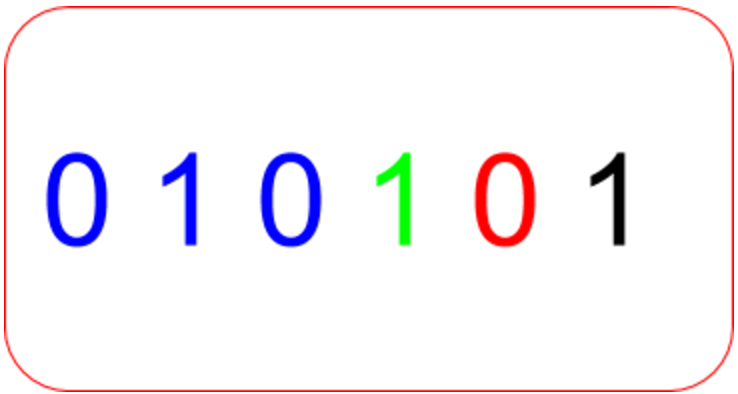
\includegraphics[width=1\textwidth]{images/state.png}
\caption{State representation for our test problem, blue digits are a one hot representation of which action the state is suggesting is correct (i.e. will yield $+1$ reward), the green digit will be 1 if and only if this state actually determines the correct action to take (i.e. it is the informant state). The red digit will be 1 if and only if the blue indicator is random and uncorrelated with the correct action choice (i.e. it is a noisy state). The final digit is simply an always on bias which may aid in the memory mechanism we will describe later. In addition to the general interpretation of these digits there is a special start node with code 000001 and the final node (at which the action choice will give a reward) with code 000011.}
\label{fig:state}
\end{figure}

\begin{figure}[!ht]
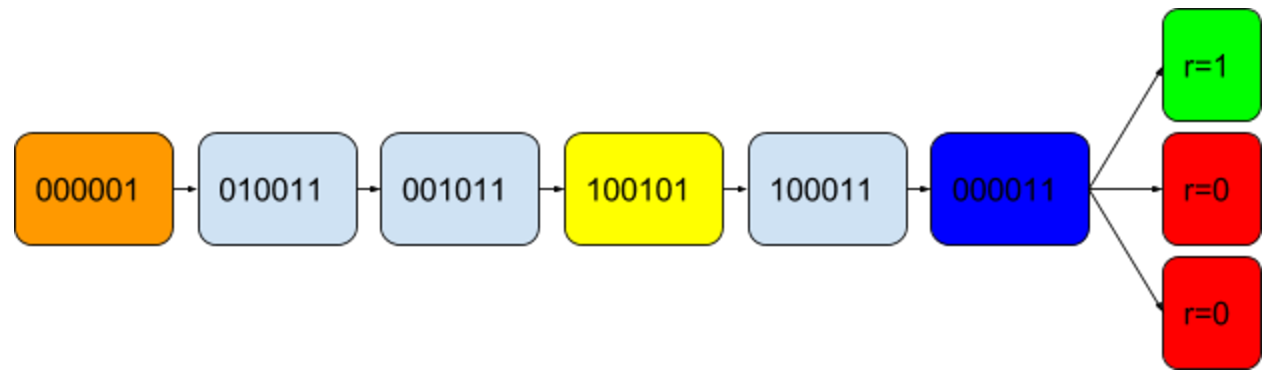
\includegraphics[width=1\textwidth]{images/problem.png}
\caption{An instance of the secret informant, the start state is orange, the final state (at which a decision must be made) is dark blue, the informant state (with the 4th bit set to 1) is yellow while the noisy states (with the 4th bit set to 0) are pale blue. Notice that because the 1st bit in the informant state is 1 and the rest are 0 the reward must be given for the top action and no other. In each instance of the problem the informant state will be placed randomly between the start and final state. Here we have 3 noisy states in addition to the informant state, in our tests we use 4 noisy states.}
\label{fig:problem}
\end{figure}

\section*{Related Work}

\section*{Proposed Method}
\begin{figure}[!ht]
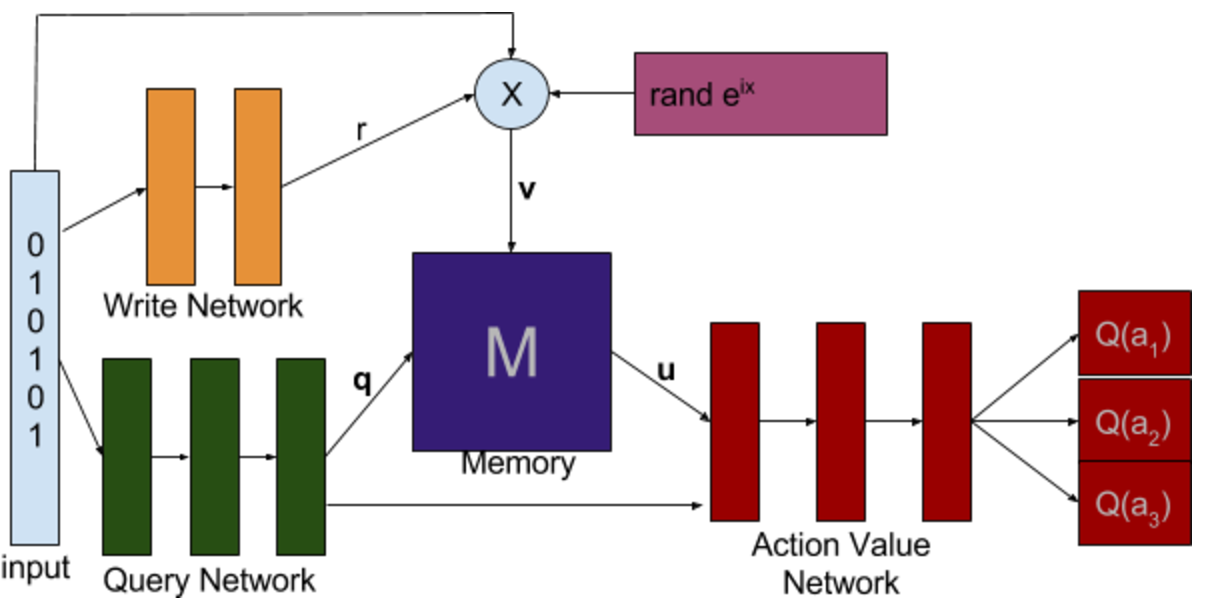
\includegraphics[width=1\textwidth]{images/architecture.png}
\caption{Our architecture, }
\label{fig:arch}
\end{figure}

\section*{Results}

\section*{Conclusion}

\section*{Future Work}


\begin{thebibliography}{plain}
\bibitem{NTM}
Graves, A., Wayne, G., and Danihelka, I. (2014) Neural Turing Machines. arXiv preprint arXiv:1410.5401.

\bibitem{MC}
Oh, J., Chockalingam, V., Singh, S., and Lee, H. (2016) Control of Memory, Active Perception, and Action in Minecraft. ICML, New York City, 2016. JMLR Workshop and Conference Proceedings Volume 48.

\bibitem{LSTM}
Danihelka, I., Wayne, G., Uria, B., Kalchbrenner, N., and Graves, A. (2016) Associative Long Short-Term Memory. ICML, New York City, 2016. JMLR Workshop and Conference Proceedings Volume 48.

\bibitem{DNC}
Graves, A. et al. (2016) Hybrid Computing Using a Neural Network with Dynamic External Memory. Nature 538, 471-476.
\end{thebibliography}



\end{document}